%!TEX root = Economics and Behaviour.tex


\section{Extensive form}

In game theoretic view the strategic and the extensive form are merely two different representations of the same strategic decision situation. But while the strategic form often only provides a static description of a game, the extensiv form provides additional properties like move order or level of information in a game.

\begin{example}[Dictator-Game] \index{Dictator-Game}
Image two players, a proposer $P$ can split up 10 \euro ~ (up to \euro-level) between him and a receiver $R$. 
	\begin{itemize}
		\item Question 1: Assume for a minute $P$ is totally selfish and only cares about his own profits. Is there a strictly dominant strategy for $P$? \\
			Yes! $(10, 0)$ (money proposer, money receiver) is strictly dominant.
		\item Question 2: What if $P$ is a pure altruist and just cares about the money $R$ receives? \\
			Then $(0, 10)$ is strictly dominant.
	\end{itemize}
\end{example}

This simply example for a game we are now going to extend into a dynamic game with the addition that after the proposal the receiver can depending on the offer either accept or reject the proposal.

An extensive form is suitable to model games like this and  we will find later not far to seek that it often has the form a a tree. The definition of a game in extensive form consists of:
\begin{itemize} \index{extensive form}
	\item A finite set of nodes $\mathcal{X}$, a finite set of possible actions $\mathcal{A}$ and a finite set of players ${1, \dotsc, N}$
	\item A function $p \colon \mathcal{X} \rightarrow \{ \mathcal{X} \cup \emptyset \}$ specifying a single immediate predecessor of each node $x \in \mathcal{X}$; except for $x_{0}$ is the \begriff{initial node}. The immediate successor nodes of $x$ are $s(x) = p^{-1}(x)$. \\
		To have a tree structure, a predecessor can never be a successor and vice versa. The set of \begriff{terminal nodes} is $T = \{ x \in \mathcal{X}: s(x) = \emptyset \}$. All other nodes $\mathcal{X} \setminus T$ are \begriff{decision nodes}.
	\item A function $\alpha \colon \mathcal{X} \setminus \{ x_{0} \} \rightarrow \mathcal{A}$ giving the action that leads to any non-initial node $x$ from its immediate predecessor $p(x)$ with
		\[ x', x'' \in s(x); x' \neq x'' \Rightarrow \alpha(x') \neq \alpha(x''). \]
		The set of choices at decision node $x$ is $c(x) = \{ a \in \mathcal{A} : a = \alpha(x')$ for some $x' \in s(x) \}$
	\item A collection of information sets $\mathcal{H}$, and a function $H : \mathcal{X} \rightarrow \mathcal{H}$, assigning each decision node $x$ to an information set $H(x) \in \mathcal{H}$ with $c(x) = c(x')$ if $H(x) = H(x')$.
		The choices available at information set $H$ can be written as
		\[ C(H) = \{a \in A : a \in c(x) \text{ for } x \in H \}. \]
	\item A function $\tau : \mathcal{H} \rightarrow \{0, 1, \dotsc, N \}$ assigning a player to each information set ($i = 0$ 'nature').
		The collection of player $i$'s information set is denoted by $\mathcal{H}_i = \{H \in \mathcal{H} : i = \tau(H) \}$.
	\item A function $\rho : \mathcal{H}_{0} \times \mathcal{A} \rightarrow [0, 1]$ assigning a probability to each action of nature with $ \rho (H,a) = 0$ if $a \notin C(H)$ and $\sum_{a \in C(H)} \rho(H,a) = 1$ for all $H \in \mathcal{H}_{0}$.
	\item A collection of payoff functions $u = \{ u_{1}(\dotsc), \dotsc, u_{N} (\dotsc) \}$, where $u_{i} \colon T \rightarrow \mathds{R}$.
\end{itemize}

Now, back to our example:

\begin{example}[Ultimatum-Game]	\label{ultimatumgame} \index{Ultimatum-Game} 
Given two players one of them, the proposer $P$, receives a sum of money ($M = 10$) and decides how to divide the sum between himself and another player, the receiver $R$, where $P$ receives $(x_{p})$ (with $x_{p} \in \{ 0, 1, 2, \dotsc, 10 \}$) and $R$ collects $(10 - x_{p})$. After the proposer's decision the responder can either accept or reject this offer, if he accepts the money is split according to the proposal if he rejects neither player receives any money.

To sum it up:
	\begin{itemize}
		\item $P$ proposes split up $(x_{p}, 10 - x_{p})$
		\item $R$ accepts or rejects
			\begin{itemize}
				\item If $R$ accepts $(a)$ proposal becomes implemented. $P$ receives $x_{p}$ and R $10 - x_{p}$
				\item If $R$ rejects $(r)$ the payout for both players is $0$.
			\end{itemize}
	\end{itemize}
	
	\begin{center}
		\begin{tikzpicture}[auto, level distance=30mm, sibling distance=35mm]
			\node [circle,draw] (z){$P$}
 						child {node [circle,draw] (a) {$10$}	}
 						child {node [] (b) {$ $}	}
 						child {node [circle,draw] (c) {$x_{p}$}
  							child {node [circle,draw] (f) {$(x_{p}, 10 - x_{p})$}	}
  			 				child {node [circle,draw] (g) {$(0, 0)$}	}			
 						}
 						child {node [] (d) {$$}	}
  						child {node [circle,draw] (e) {$0$}
			};
			\path (a) -- (b) node [midway] {$\dotsc$};
			\path (b) -- (c) node [midway] {$\dotsc$};
			\path (c) -- (d) node [midway] {$\dotsc$};
			\path (d) -- (e) node [midway] {$\dotsc$};
			\path (f) -- (g) node [midway] {$a$ $/$ $r$};
		\end{tikzpicture}				
	\end{center}
	
	A strategy set in this game, as it needs to specify a complete action plan, would have to look similar to
	\begin{itemize}
		\item Proposer sets a $x_{p}$
		\item Receiver decides for \textit{any} $x_{p}$ that might come up if he'd accept or reject that offer.
	\end{itemize}
	
	\textbf{1. Question:} Can the outcome $(5, 5)$ be stabilised as a Nash-Equilibrium? \\
	\textbf{Answer:} Yes. Say P proposes $x_{p} = 5$ and the strategy set for R is defined by accepting for any value of $x_{p} \leq 5$ and rejecting the offer for values larger than $5$. \\
		In this situation $(5, 5)$ would be stabilised as a Nash-Equilibrium.


	\textbf{2. Question:} Is there another Nash-Equilibrium that stabilises the $(5, 5)$ outcome? \\
	\textbf{Answer:} Yes. If P again proposes $x_{p} = 5$ and the strategy set for R is defined by accepting for only $x_{p} = 5$ and rejecting for any other case, so $x_{p} \neq 5$. 
	
	
	\textbf{3. Question:} Can $(0, 10)$ be stabilised as a Nash-Equilibrium? \\
	\textbf{Answer:} Yes. We set the strategy for P as $x_{p} = 0$ and for R demand accepting for $x_{p} = 0$ and rejecting for any other case, meaning for $x_{p} \geq 1$. 
\end{example}
As we can see the Nash-Equilibrium can lead to an infinite amount of outcomes some of them even with implausible threats. We'd therefore like to refine this kind of equilibrium which leads us to the (sub-game) perfect Nash-Equilibrium.

\begin{definition}[Sub-game] \index{sub-game}
	A sub-game is any part of a game that meets the following criteria:
	\begin{itemize}
		\item It has a single initial node that is the only member of that node's information set (i.e. the initial node is in a singleton information set).
		\item If a node is contained in the sub-game then so are all of its successors
		\item If a node in a particular information set is in the sub-game then all members of that information set belong to the sub-game.
		\item and finally the node must not contain a deterministic state but instead at least one non-trivial choice
	\end{itemize}
\end{definition}

\begin{definition}[(Sub-game-)Perfect Nash-Equilibrium] \index{Sub-game-Perfect Nash-Equilibrium} 
A strategy profile is a Sub-game-Perfect Nash-Equilibrium if it represents a Nash equilibrium of every sub-game of the original game. Informally, this means that if the players played any smaller game that consisted of only one part of the larger game and their behaviour represents a Nash equilibrium of that smaller game, then their behaviour is a sub-game perfect equilibrium of the larger game. 
\end{definition}

How to find a Perfect Nash-Equilibrium:
\begin{enumerate}
	\item Define (one set of) optimal actions for the last sub-game
	\item Replace that decision nodes with the respective outcome
	\item Repeat $(1)$ and $(2)$ until the initial decision node.
\end{enumerate}

\begin{example}[Sequel to the Ultimatum-Game]
	Searching for the Perfect Nash-Equilibrium in this case leads to:
	\begin{enumerate}
		\item Defining the optimal actions
			\begin{itemize}
				\item In the case $P$ offering $0$ ($x_{p} = 10$), $R$ receives nothing and is therefore indifferent between refusing and accepting. Let's assume for now he'd accept.
				\item For $x_{p} \in [0, 10)$ $R$ always has to accept the offer since $10 - x_{p} > 0$.
			\end{itemize}
		\item Assuming $R$ always accepts, we now can reduce the game to
			\begin{center}
				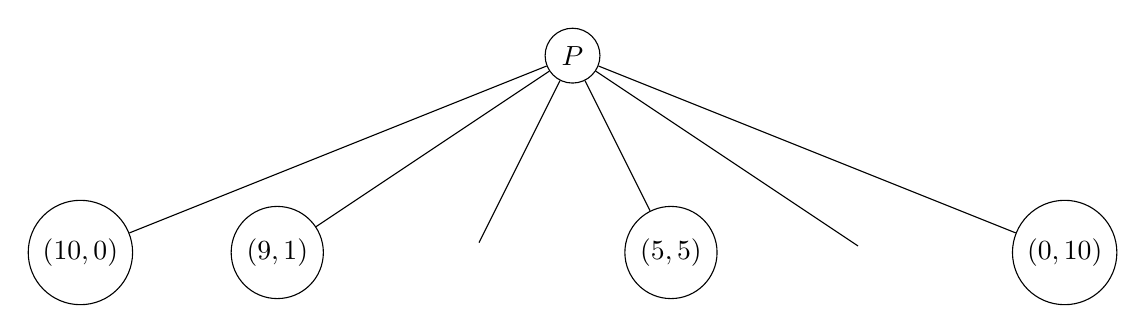
\begin{tikzpicture}[level/.style={sibling distance=25mm/#1}, level 	distance=25mm]
					\node [circle,draw] (z){$P$}
 						child {node [circle,draw] (a) {$(10, 0)$}	}
 						child {node [circle,draw] (b) {$(9, 1)$}	}
 						child {node [] (c) {$ $}	}
 						child {node [circle,draw] (d) {$(5, 5)$}	}
 						child {node [] (e) {$ $}	}
  						child {node [circle,draw] (f) {$(0, 10)$}
					};
					\path (b) -- (c) node [midway] {$\dotsc$};
					\path (c) -- (d) node [midway] {$\dotsc$};
					\path (d) -- (e) node [midway] {$\dotsc$};
					\path (e) -- (f) node [midway] {$\dotsc$};
				\end{tikzpicture}				
			\end{center}
		\item A simple search in the reduced game tree for the strategy with the highest expected payoff for $P$ yields the Sub-Game-Perfect Nash-Equilibrium as we have reached the initial node.
	\end{enumerate}
	$\Rightarrow P$ playing $x_{p} = 10$ together with $R$ always accepting constitutes a Sub-game-Perfect Nash-Equilibrium. 

	Now changing our assumption about player $R$'s decision in case of the offer $0$ leads to
			\begin{itemize}
				\item Again, for $x_{p} \in [0, 10)$ $R$ receives $10 - x_{p} > 0$, therefore he'd have to accept the offer in these situations.
				\item For the remaining offer $0$ ($x_{p} = 10$), it would be just as plausible to refuse the offer, since he is indifferent between both choices. Hence, accepting for $x_{p} \in [0, 10)$ and refusing for $x_{p} = 10$ is also a sub-game perfect strategy.
			\end{itemize}
		 and even if the tree changes only slightly a different Sub-game-Perfect Nash-Equilibrium occurs:
			\begin{center}
				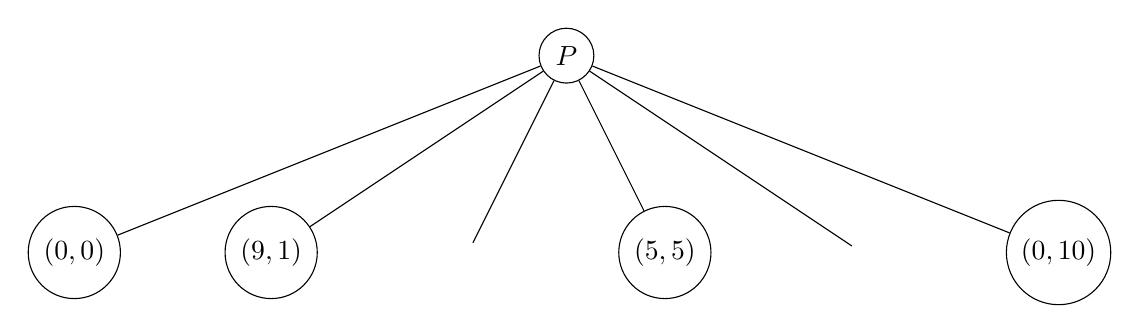
\begin{tikzpicture}[level/.style={sibling distance=25mm/#1}, level 	distance=25mm]
					\node [circle,draw] (z){$P$}
 						child {node [circle,draw] (a) {$(0, 0)$}	}
 						child {node [circle,draw] (b) {$(9, 1)$}	}
 						child {node [] (c) {$ $}	}
 						child {node [circle,draw] (d) {$(5, 5)$}	}
 						child {node [] (e) {$ $}	}
  						child {node [circle,draw] (f) {$(0, 10)$}
					};
					\path (b) -- (c) node [midway] {$\dotsc$};
					\path (c) -- (d) node [midway] {$\dotsc$};
					\path (d) -- (e) node [midway] {$\dotsc$};
					\path (e) -- (f) node [midway] {$\dotsc$};
				\end{tikzpicture}				
			\end{center}
	$\Rightarrow P$ playing $x_{p} = 9$ together with $R$ always accepting if $x_{p} < 10$ and refusing for $x_{p} = 10$ also constitutes a Sub-game-Perfect Nash-Equilibrium. 
\end{example}



\newpage